\documentclass[border=2mm]{standalone}

\usepackage{pgfplots}
\pgfplotsset{compat=1.18}
\usetikzlibrary{arrows.meta, 
  calc, 
  positioning, 
  decorations.pathreplacing, 
  calligraphy}

\usepackage{xcolor}
\definecolor{den-1}{HTML}{111111}   % Đen #111111
\definecolor{den-2}{HTML}{222222}   % Đen #222222
\definecolor{den-3}{HTML}{333333}   % Đen #333333
\definecolor{den-4}{HTML}{444444}   % Đen #444444
\definecolor{den-5}{HTML}{555555}   % Đen #555555
\definecolor{den-6}{HTML}{666666}   % Đen #666666

% Thiết lập vị trí đặt nhãn gốc tọa độ
\tikzset{
  >=Stealth,
  originlabel/.style={
    font=\small\sf,
    anchor=north east, % Vị trí tương đối so với gốc
    yshift=-0.1ex,     % Điều chỉnh vị trí dọc một chút
    xshift=-0.1ex      % Điều chỉnh vị trí ngang một chút
  }
}

\begin{document}

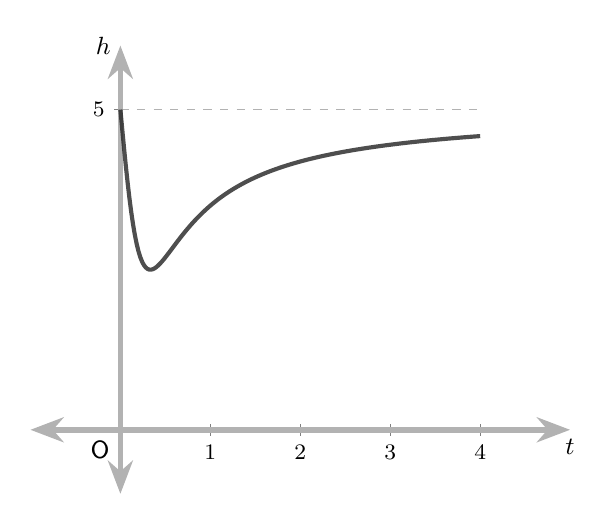
\begin{tikzpicture}

\begin{axis}[
    font=\small\sf,
    axis lines=middle,
    axis line style={<->, line width=2pt, color=den-6!50},
    xlabel=$t$, ylabel=$h$,
    xlabel style={below, font=\small\sf},
    ylabel style={left, font=\small\sf},
    xmin=-1, xmax=5,
    ymin=-1, ymax=6,
    xtick={1,2,3,4},
    ytick={5},
    tick label style={font=\footnotesize\sf, /pgf/number format/use comma=false, /pgf/number format/1000 sep={}},
    clip=false,
]

\node[originlabel] at (axis cs:0,0) {O};

\draw [dashed, color=den-6!50] (0,5) -- (4,5);

\addplot[domain=0:4, samples=200, line width=1.5pt, color=den-2, opacity=.8] {5-(15*x)/(9*x^2+1)};

\end{axis}

\end{tikzpicture}

\end{document}